\tableofcontents
\section*{Предисловие}
При выполнении данной лабораторной работы было решено использовать 
\href{https://python-control.readthedocs.io/en/0.9.4/}{Python Control Systems Library}.
Данный инструмент является альтернативой Matlab, адаптированной для использования на 
языке Python и предоставляет широкий функционал для анализа и моделирования систем,
а также синтеза регуляторов для управления.

Полный листинг моделирования систем представлен в \href{https://github.com/diuzhevVlad/control-theory-itmo-fall-2023/blob/main/Lab10/Lab10.ipynb}{jupyter notebook} на GitHub.

\pagebreak

\section{Исследование LQR}
В лабораторной работе будем использовать следующие матрицы системы:
\begin{equation*}
    A = \begin{bmatrix}
        6 & 26 & 4 & 17 \\
        0 & 9 & 0 & 6 \\
        -10 & -35 & -6 & -25 \\
        0 & -15 & 0 & -9
    \end{bmatrix},
    B = \begin{bmatrix}
        7 & 0 \\
        2 & 0 \\
        -10 & 0 \\
        -4 & 0
    \end{bmatrix},
    C = \begin{bmatrix}
        4 & 0 & 2 & 2 \\
        0 & 12 & 0 & 6
    \end{bmatrix},
    D = \begin{bmatrix}
        0 & 0 \\
        0 & 3
    \end{bmatrix}
\end{equation*}
Рассмотрим систему:
\begin{equation}
    \dot{x} = Ax + Bu
\end{equation}
Для синтеза регуляторов зададимся набором матриц $Q$ и $R$:
\begin{equation*}
    Q_1 = diag(\begin{bmatrix}
        0.01 & 0.01 & 0.01 & 0.01
    \end{bmatrix}), R_1 = diag(\begin{bmatrix}
        1 & 1
    \end{bmatrix})
\end{equation*}
\begin{equation*}
    Q_2 = diag(\begin{bmatrix}
        0.1 & 0.1 & 0.1 & 0.1
    \end{bmatrix}), R_2 = diag(\begin{bmatrix}
        0.1 & 0.1
    \end{bmatrix})
\end{equation*}
\begin{equation*}
    Q_3 = diag(\begin{bmatrix}
        1 & 1 & 1 & 1
    \end{bmatrix}), R_3 = diag(\begin{bmatrix}
        0.01 & 0.01
    \end{bmatrix})
\end{equation*}
Путем решения следующих уравнение найдем матрицу регулятора:
\begin{equation}
    \begin{cases}
        A^T P + P A + Q - PBR^{-1}B^TP = 0\\
        K = -R^{-1} B^T P \\
    \end{cases}
\end{equation}
Полученные матрицы:
\begin{equation*}
    K_1 = \begin{bmatrix}
        -0.28 & -1.06 & -0.27 & -0.74 \\
        0 & 0 & 0 & 0
    \end{bmatrix}
\end{equation*}
\begin{equation*}
    K_2 = \begin{bmatrix}
        -3.83 & -14.73 & -3.2 & -9.68 \\
        0 & 0 & 0 & 0
    \end{bmatrix}
\end{equation*}
\begin{equation*}
    K_3 = \begin{bmatrix}
        -42.81 & -159.25 & -33.85 & -102.91 \\
        0 & 0 & 0 & 0
    \end{bmatrix}
\end{equation*}

Данный метод синтеза позволяет минимизировать функционал:
\begin{equation}
    J = \int_{0}^{\inf}(x^T(t)Qx(t)+u^T(t)Ru(t))dt
\end{equation}
Получив матрицу $P$ можем найти его значение аналитически:
\begin{equation}
    J_{an} = x_0^TPx_0
\end{equation}

Проведем моделирование и сравним значения функционалов:
\begin{equation*}
    J_1=14.2, J_{an1}=14.21
\end{equation*}
\begin{equation*}
    J_2=54.21, J_{an2}=54.16
\end{equation*}
\begin{equation*}
    J_3=467.1, J_{an3}=466.2
\end{equation*}

\begin{figure}[h]
    \centering
    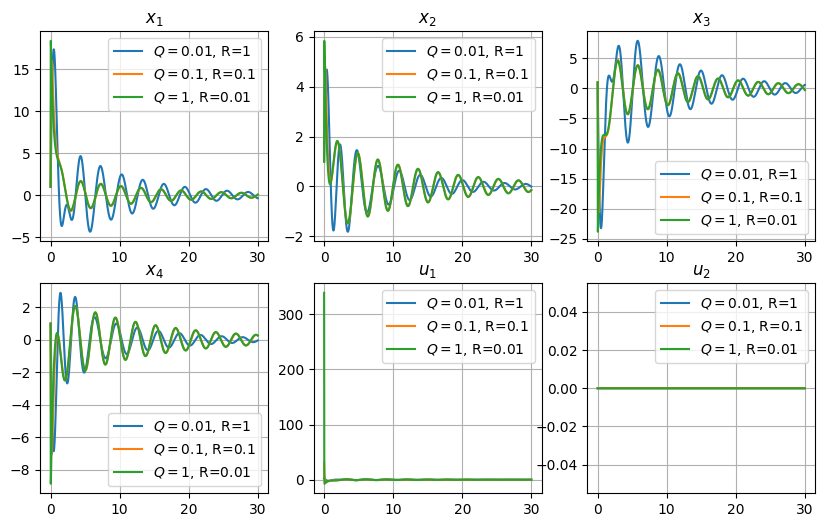
\includegraphics[width=300px]{plot_1.png}
    \caption{\label{fig:The-caption-1}Задание 1. Компоненты вектора состояний при различных матрицах $Q$ и $R$ регулятора.}
\end{figure}

\pagebreak

\section{Сравнение LQR с не-LQR}
Возьмем регулятор, соответствующий второй паре матриц $Q$ и $R$. Также синтезируем модальный регулятор
(со спетром {$-1,-1,-1,-1$}) и регулятор методом LMI (степени устойчивости $\alpha=0.1$)

Проведем моделирование систем, замкнутых данными регуляторами:
\begin{figure}[h]
    \centering
    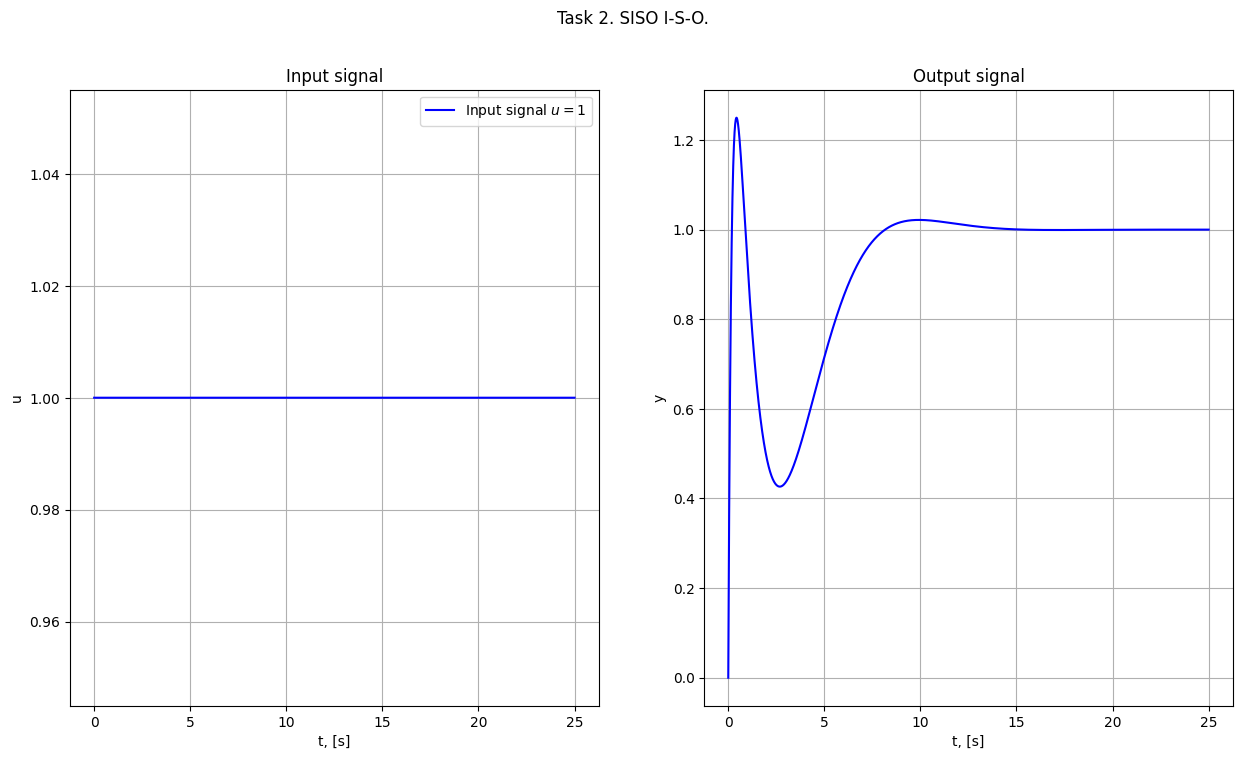
\includegraphics[width=300px]{plot_2_1.png}
    \caption{\label{fig:The-caption-2}Задание 2. Компоненты вектора состояний систем, замкнутых различными регуляторами.}
\end{figure}

Простроим график $J(t) = \int_{0}^{t}(x^T(\tau)Qx(\tau)+u^T(\tau)Ru(\tau))d\tau$:
\begin{figure}[h]
    \centering
    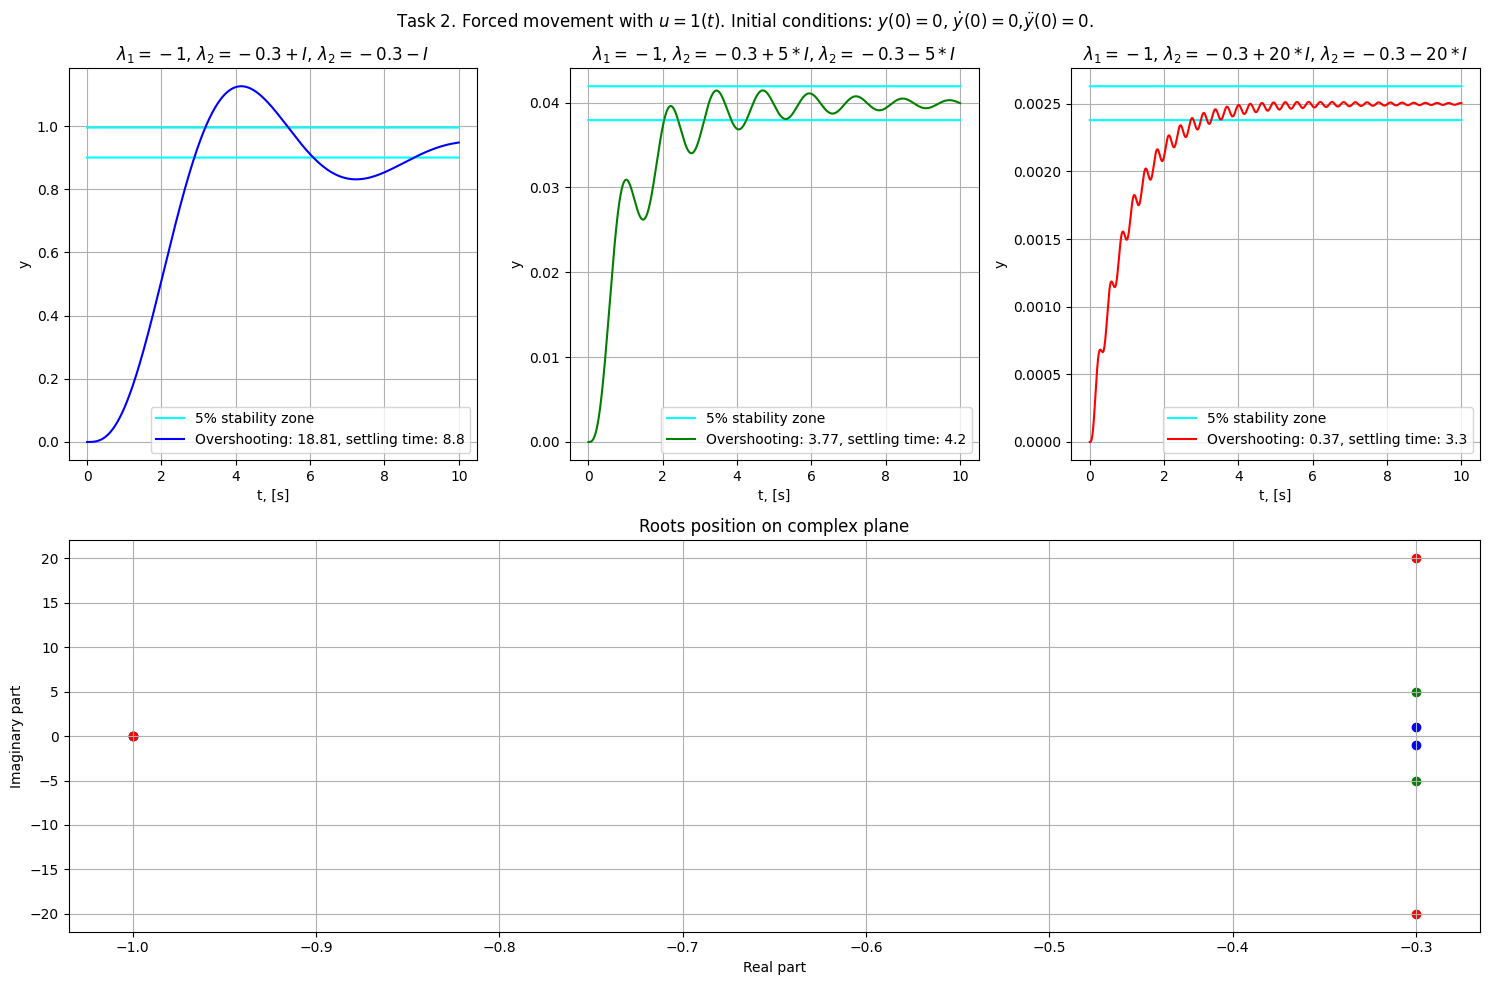
\includegraphics[width=300px]{plot_2_2.png}
    \caption{\label{fig:The-caption-2}Задание 2. Значения критерия оптимальности.}
\end{figure}
\pagebreak

\section{Исследование LQE (фильтра Калмана)}
Рассмотрим систему:
\begin{equation}
    \dot{x} = Ax + f, y = Cx + \xi
\end{equation}
Внешние возмущения $f$ и $\xi$  будем считать белым шумам с заданной дисперсией.

Путем решения следующих уравнений найдем матрицу наблюдателя:
\begin{equation}
    \begin{cases}
        A P + P A^T + Q - PC^TR^{-1}CP = 0\\
        L = -PC^TR^{-1} \\
    \end{cases}
\end{equation}
Проведем исследования работы наблюдателя при различных параметрах внешних воздействий и матрицах $Q$ и $R$:

\begin{figure}[]
    \centering
    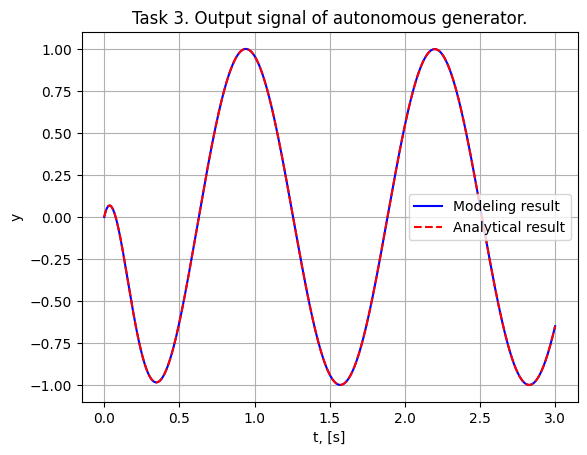
\includegraphics[width=300px]{plot_3_1.png}
    \caption{\label{fig:The-caption-1}Задание 3. Компоненты вектора состояний и выход системы наблюдателя.}
\end{figure}
\begin{figure}[]
    \centering
    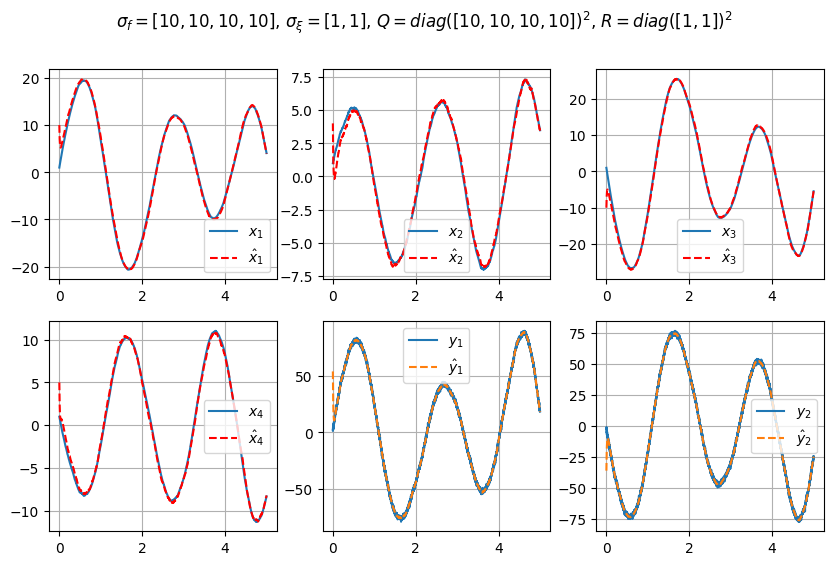
\includegraphics[width=300px]{plot_3_2.png}
    \caption{\label{fig:The-caption-1}Задание 3. Компоненты вектора состояний и выход системы наблюдателя.}
\end{figure}
\begin{figure}[]
    \centering
    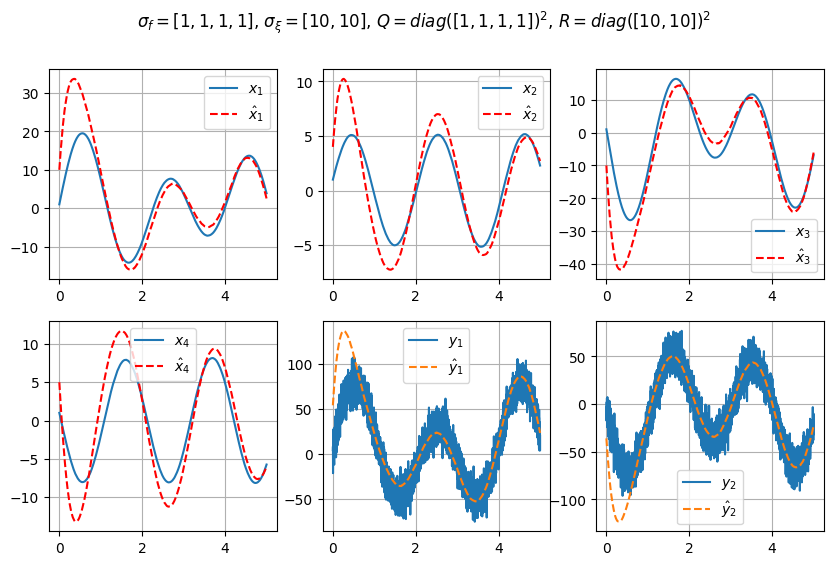
\includegraphics[width=300px]{plot_3_3.png}
    \caption{\label{fig:The-caption-1}Задание 3. Компоненты вектора состояний и выход системы наблюдателя.}
\end{figure}
\begin{figure}[]
    \centering
    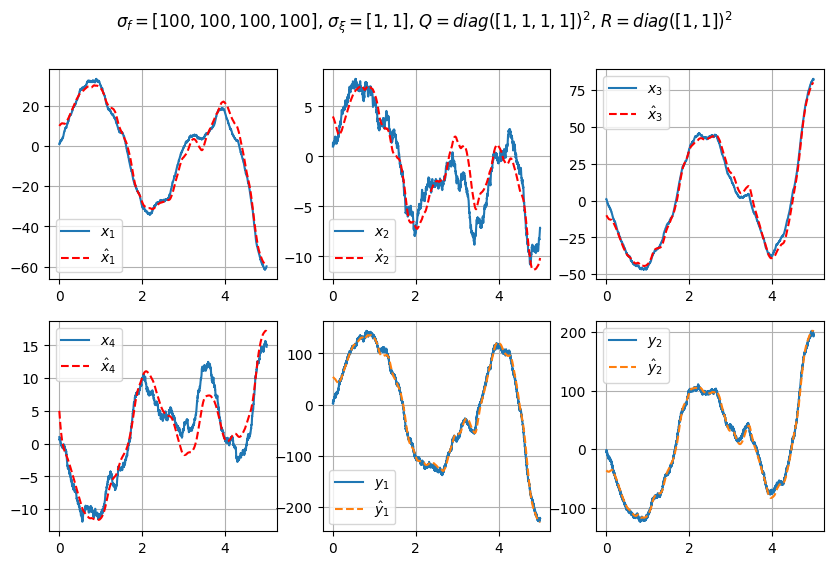
\includegraphics[width=300px]{plot_3_4.png}
    \caption{\label{fig:The-caption-1}Задание 3. Компоненты вектора состояний и выход системы наблюдателя.}
\end{figure}
\begin{figure}[]
    \centering
    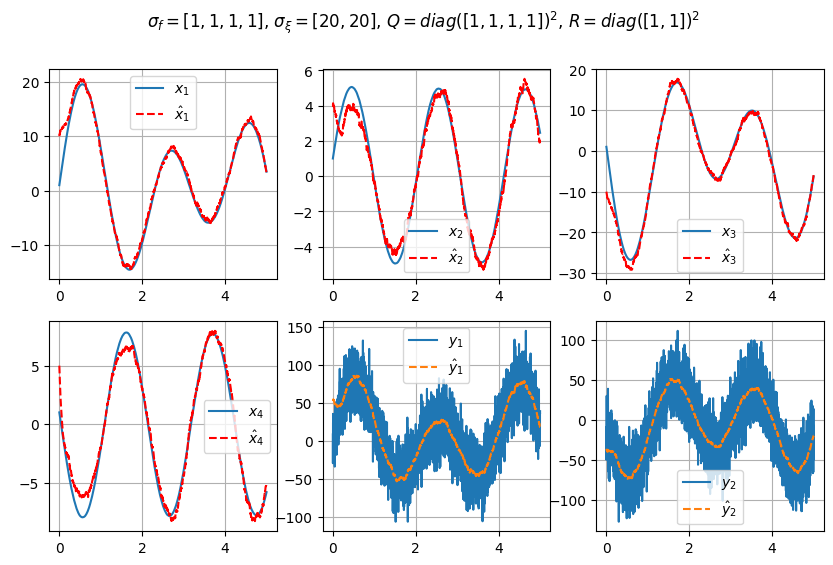
\includegraphics[width=300px]{plot_3_5.png}
    \caption{\label{fig:The-caption-1}Задание 3. Компоненты вектора состояний и выход системы наблюдателя.}
\end{figure}
\begin{figure}[]
    \centering
    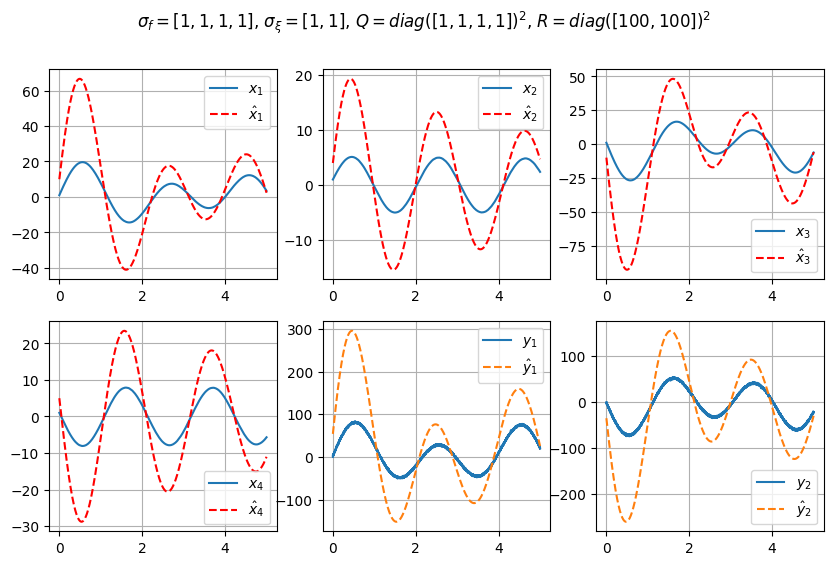
\includegraphics[width=300px]{plot_3_6.png}
    \caption{\label{fig:The-caption-1}Задание 3. Компоненты вектора состояний и выход системы наблюдателя.}
\end{figure}
\begin{figure}[]
    \centering
    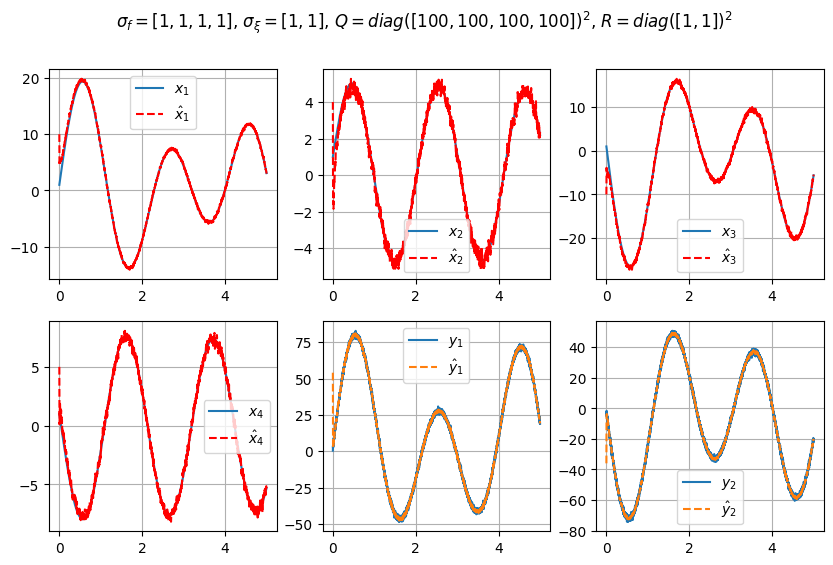
\includegraphics[width=300px]{plot_3_7.png}
    \caption{\label{fig:The-caption-1}Задание 3. Компоненты вектора состояний и выход системы наблюдателя.}
\end{figure}
\begin{figure}[]
    \centering
    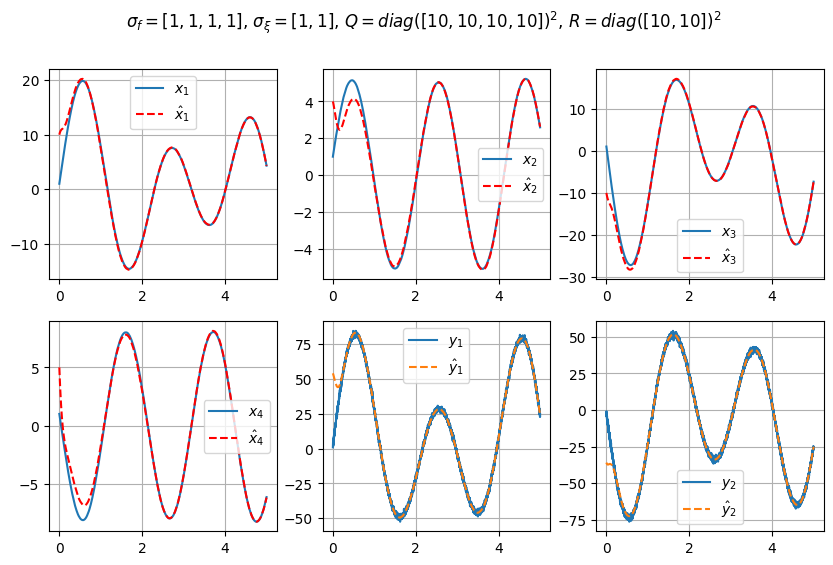
\includegraphics[width=300px]{plot_3_8.png}
    \caption{\label{fig:The-caption-1}Задание 3. Компоненты вектора состояний и выход системы наблюдателя.}
\end{figure}
\pagebreak

\section{Синтез LQG}
Рассмотрим систему с регулятором и наблюдателем:
\begin{equation}
    \begin{cases}
        \dot{x} = Ax + BK\hat{x} + f \\
        y = Cx + DK\hat{x} + \xi \\
        \dot{\hat{x}} = A\hat{x} + BK\hat{x} + L(\hat{y}-y) \\
        \hat{y} = C\hat{x} + DK\hat{x}
    \end{cases}
\end{equation}
Введя величину ошибки наблюдателя $(e = x - \hat{x})$, получим эквивалентную систему:
\begin{equation}
    \begin{bmatrix}
        \dot{x} \\ \dot{e}
    \end{bmatrix} =
    \begin{bmatrix}
        A + BK & -BK \\
        \Theta_{n \times n} & A + LC
    \end{bmatrix}
    \begin{bmatrix}
        x \\ e
    \end{bmatrix} +
    \begin{bmatrix}
        I_{n \times n} & \Theta_{n \times m} \\
        I_{n \times n} & L
    \end{bmatrix}
    \begin{bmatrix}
        f \\ \xi
    \end{bmatrix}
\end{equation}

Зададимся значениями стандартных отклонений для распределений внешних воздействий: $f_i \sim N(0,3^3) $, $\xi \sim N(0,5^2)$.
Соответствующим образом выбрав матрицы $Q$ и $R$ синтезируем LQE и LQR:
\begin{figure}[h]
    \centering
    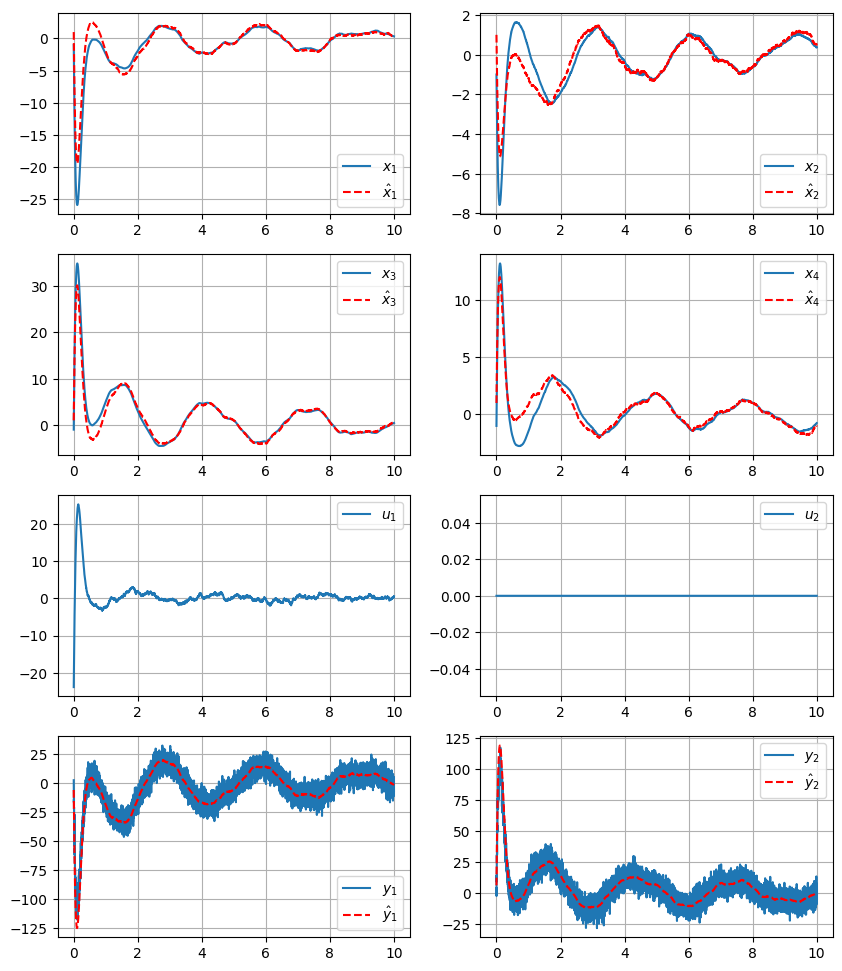
\includegraphics[width=300px]{plot_4.png}
    \caption{\label{fig:The-caption-1}Задание 4. Компоненты вектора состояний, управление и выход системы с LQG.}
\end{figure}
\pagebreak

\section{Выводы}\
\begin{enumerate}
    \item Выбирая матрицы параметров $Q$ и $R$ можно задавать оптимальный критерий, который минимизируют при своем исполнении LQE и LGR.
    \item Убедились в том, что LQR действительно предоставляет оптимальное значение коэффициентов по сравнению с другими способами синтеза.
    \item При правильной настройке параметров наблюдателя, LQE способен сглаживать сигнал и восстанавливать вектор состояний системы с большой точностью не смотря на шумы. Заметим, однако, что при меньших значениях шума наблюдатель демонстрирует лучшую сходимость.
    \item Независимо синтезированные LQE и LQR можно объединить в одну систему.
\end{enumerate}